%%%%%%%%%%%%%%%%%%%%%%%%%%%%%%%%%%%%%%%%%%%%%%%%%%%%%%%%%%%%%%%%%%%%%%%%
% Preamble
%%%%%%%%%%%%%%%%%%%%%%%%%%%%%%%%%%%%%%%%%%%%%%%%%%%%%%%%%%%%%%%%%%%%%%%%
\documentclass[11pt]{article}
%
% Packages and other includes
% Pagination
\usepackage[letterpaper, margin=1in]{geometry}
\usepackage{emptypage}
%
% Fonts
\usepackage[T1]{fontenc} % best for Western European languages
\usepackage{lmodern} % Latin Modern instead of CM
\usepackage{textcomp} % required to get special symbols
%
% Math
\usepackage{amsmath, amssymb}
\usepackage{braket}
%
% Graphics, floats, tables
\usepackage{graphicx, color, float, array}
%
% Hyperlinks
\usepackage{hyperref}
%
%
% Definitions and settings
% Paragraph indent and spacing
\setlength{\parskip}{0.4\baselineskip}
\setlength{\parindent}{0in}
%
%
% Title, authors, date
\title{\textbf{Midterm answers}}
%
%
%%%%%%%%%%%%%%%%%%%%%%%%%%%%%%%%%%%%%%%%%%%%%%%%%%%%%%%%%%%%%%%%%%%%%%%%
% Main document
%%%%%%%%%%%%%%%%%%%%%%%%%%%%%%%%%%%%%%%%%%%%%%%%%%%%%%%%%%%%%%%%%%%%%%%%
%

\begin{document}

\maketitle

1. a) $8.50*10^3$ meters

b) Overestimation. A potential error is that deriving the barometric formula assumes
a constant temperature. This is not true in reality since temperature decreases
going higher in altitude.

c) P(O$_2$)=53.1 torr, around 75$\%$ Hb saturation

2. a)

\begin{center}
  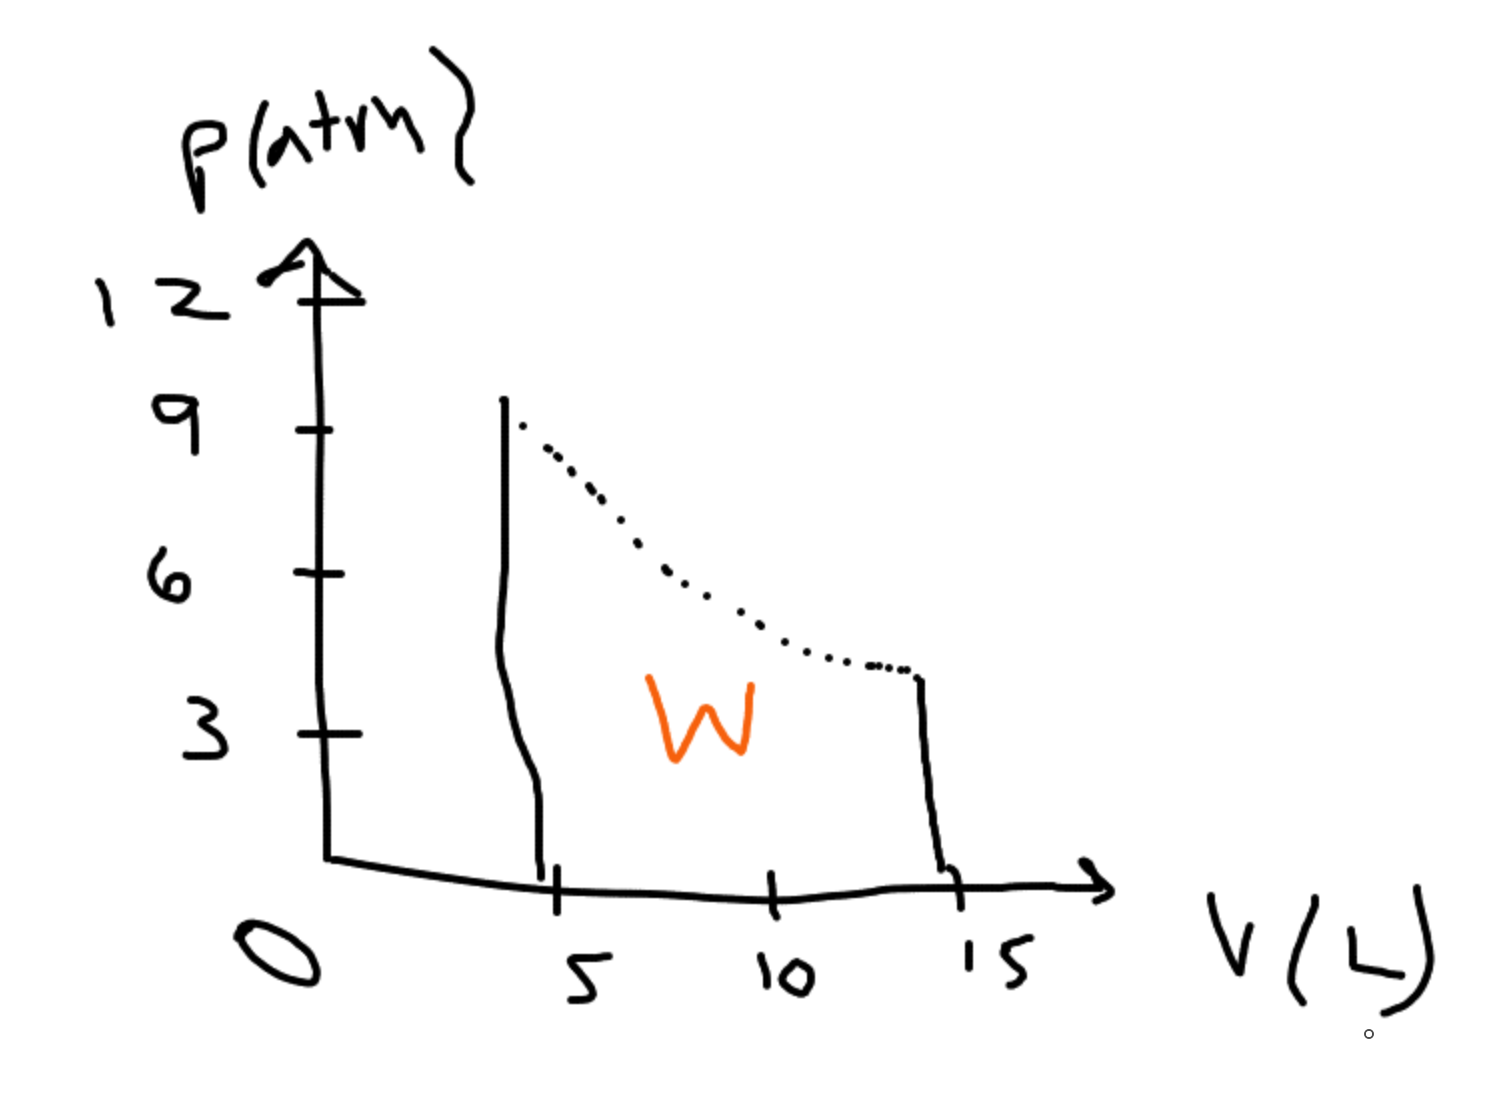
\includegraphics[scale=0.15]{sketch.png}
\end{center}

b) $W = -nRT\ln \frac{V_f}{V_i} =  5470\text{J/mol}$ and $Q=-5470\text{J/mol}$

c) $P= nRT/V_f = 9.87\text{atm}$

3. The world energy crisis is the depletion of fossil fuels or nonrenewable
resources. This is imprecise because energy is neither created nor destroyed based
on 1st of thermodynamics. The energy crisis is related to global warming due the
increase in greenhouse gases such as CO$_2$ leading to less heat escaping the
atmosphere.

4. a) S$_8$(s) + 8 O$_2$(g) $\rightarrow$ 8 SO$_2$(g)

b) $Q = C\Delta T = -530*(304.7 - 296) = -4.611\text{kJ}$

c) $\Delta H_r = \frac{Q}{n_r} = \frac{-4.611}{1/(8*32.05)} -1183\text{kJ/mol}$

d) $\Delta H^\circ_f = -147.8\text{kJ/mol}$

(These values are off by a factor of 2. Need to double the $\Delta T$ or $C$)

5. $m_h$ is mass (kg) of hot bath, $m_c$ is the mass (kg) of the cold tap water, $C$ is
heat capacity of water and $\Delta T$ is the change in temperature

\begin{align}
  m_h C \Delta T_h & = m_c C \Delta T_c \\
  m_h \Delta T_h & = m_c \Delta T_c \\
  -283.0543*(40 - 43.3333) & = m_c (40 - 10) \\
  m_c = 31.450446
\end{align}

The volume needed is 8.332 galllons of $50^\circ\text{F}$

\pagebreak

\end{document}
